
\documentclass{report}

\usepackage[utf8]{inputenc}
\usepackage[italian]{babel}
\usepackage{import}
\usepackage{todonotes}
\usepackage{color}
\usepackage{rotating}
\usepackage[hidelinks]{hyperref}
\usepackage{url}
\usepackage{pdfpages}
\usepackage{siunitx}
\usepackage{pdflscape}
\usepackage{subfig}
\usepackage[euler]{textgreek}

\usepackage{enumerate} 
\usepackage{amsmath}
\usepackage{amsfonts}

\usepackage[signatures,swapnames,sans]{frontespizio}

\usepackage{geometry}
\geometry{portrait, margin=3cm}
\usepackage{siunitx}
\usepackage{booktabs}

\renewcommand*\figurename{Figura}

\newcommand{\sub}[1]{\textsubscript{#1}}
\newcommand{\super}[1]{\textsuperscript{#1}}

\newcommand{\Fig}[0]{Fig.}

\usepackage{titlesec}

\titleformat{\chapter}{\normalfont\huge}{}{20pt}{\huge\bfseries}

\linespread{1.1}

\begin{document}
\addtocounter{chapter}{-1}
	\begin{frontespizio}
		\Margini{3cm}{3cm}{3cm}{3cm}
		\Universita{Bergamo}
		\Logo[43.332mm]{unibg-mark}
		\Divisione{Scuola di Ingegneria}
		\Corso[Laurea Magistrale]{Ingegneria Informatica}
		\Titolo{Elettronica e Misure Industriali}
		\Sottotitolo{Relazione esperienze di laboratorio}
		\Punteggiatura{}
		\NRelatore{Prof.}{Prof.}
		\Relatore{Valerio Re}
		\NCorrelatore{Prof.}{Prof.}
		\Correlatore{Massimo Manghisoni}
		\Candidato[1058231]{Giulia Allievi}
		\Annoaccademico{2021--2022}
		\begin{Preambolo*}
			\usepackage[italian]{babel}
			\usepackage[T1]{fontenc}
			\usepackage[utf8]{inputenc}
			\usepackage{microtype}
			\usepackage{lmodern}
			\graphicspath{{img/}}
			
			\renewcommand{\frontinstitutionfont}{\fontsize{14}{17}\bfseries\scshape}
			\renewcommand{\fronttitlefont}{\fontsize{17}{21}\bfseries\scshape}
			\renewcommand{\frontfootfont}{\fontsize{12}{14}\bfseries\scshape}
		\end{Preambolo*}
	\end{frontespizio}



%----------------------------------------------------------------------------------------
%	PAGINA BIANCA
%----------------------------------------------------------------------------------------
\newpage
\null
\thispagestyle{empty}
\newpage

%----------------------------------------------------------------------------------------
%	INDICE
%----------------------------------------------------------------------------------------
\tableofcontents

%----------------------------------------------------------------------------------------
%	PAGINA BIANCA
%----------------------------------------------------------------------------------------
\newpage
\null
\newpage

%----------------------------------------------------------------------------------------
%	INTRO
%----------------------------------------------------------------------------------------
\chapter{Introduzione}
Nelle esperienze di laboratorio si sono realizzati ed analizzati i seguenti circuiti:
\begin{itemize}
\item Esperienza 1: Emitter follower con alimentazione duale; 
\item Esperienza 2: Emitter follower con alimentazione singola; 
\item Esperienza 3: Common emitter amplifier con alimentazione duale e singola; 
\item Esperienza 4: Amplificatore invertente ed integratore con 	\textmu A741.
\end{itemize}
La relazione è suddivisa per tipologia di circuito.
%----------------------------------------------------------------------------------------
%	CIRCUITO 1: EMITTER FOLLOWER	
%----------------------------------------------------------------------------------------
\chapter{Circuito 1: Emitter Follower}
\section{Introduzione} 
Il primo circuito realizzato è l'\textit{Emitter follower}, detto anche \textit{Common collector}. Questo circuito ha un guadagno unitario, infatti la tensione misurata in uscita è uguale alla tensione applicata in ingresso, perciò si comporta come un buffer. Ne abbiamo realizzate due diverse versioni, una con alimentazione duale ed una con alimentazione singola. 
\section{Prima versione} % alimentazione duale
La prima versione di \textit{Emitter follower} analizzata è quella ad alimentazione duale. Di seguito si riportano lo schema, l'analisi del punto di lavoro e di piccolo segnale, e le misure effettuate su questo circuito. 
\begin{figure}[h]
\centering
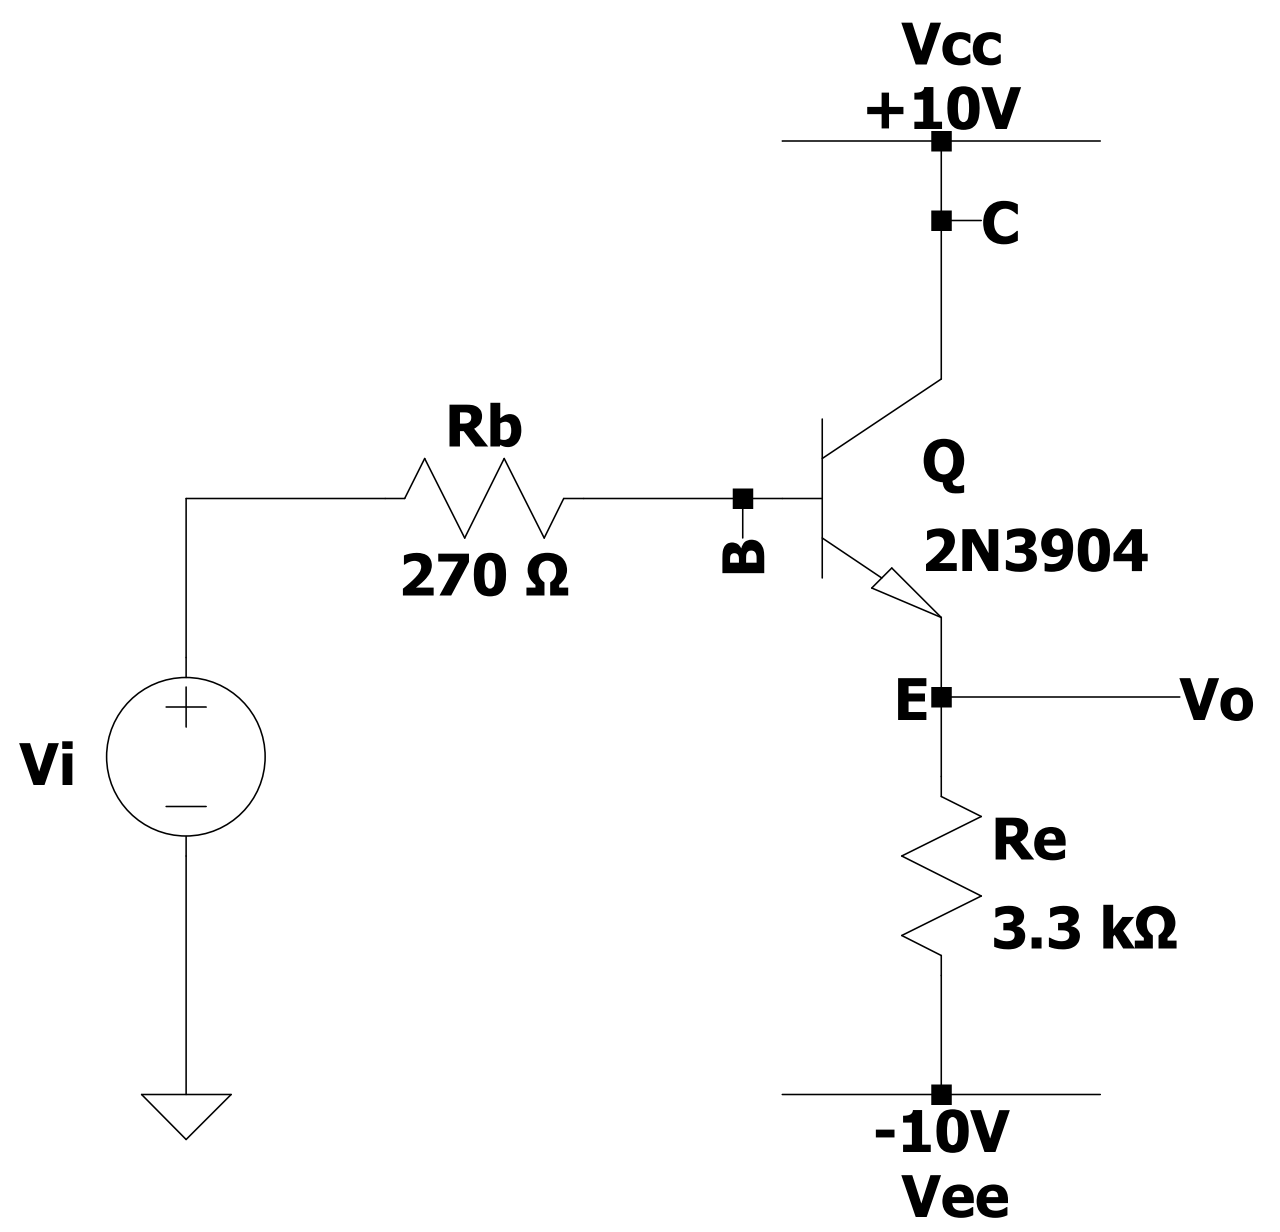
\includegraphics[height=10cm]{immagini/EFv1}
\caption{Schema dell'\textit{Emitter follower} ad alimentazione duale.}
\end{figure}
\subsection{Punto di lavoro} \label{puntolavoroEFv1}
In quest'analisi bisogna spegnere i generatori di segnale e sostituirli con un cortocircuito se sono generatori di tensione, oppure con un circuito aperto se sono generatori di corrente. I condensatori sono sostituiti con un circuito aperto e gli induttori con un cortocircuito. Successivamente si va a determinare la tensione di ogni nodo e la corrente che scorre in ogni ramo. 
\begin{figure}[h]
\centering
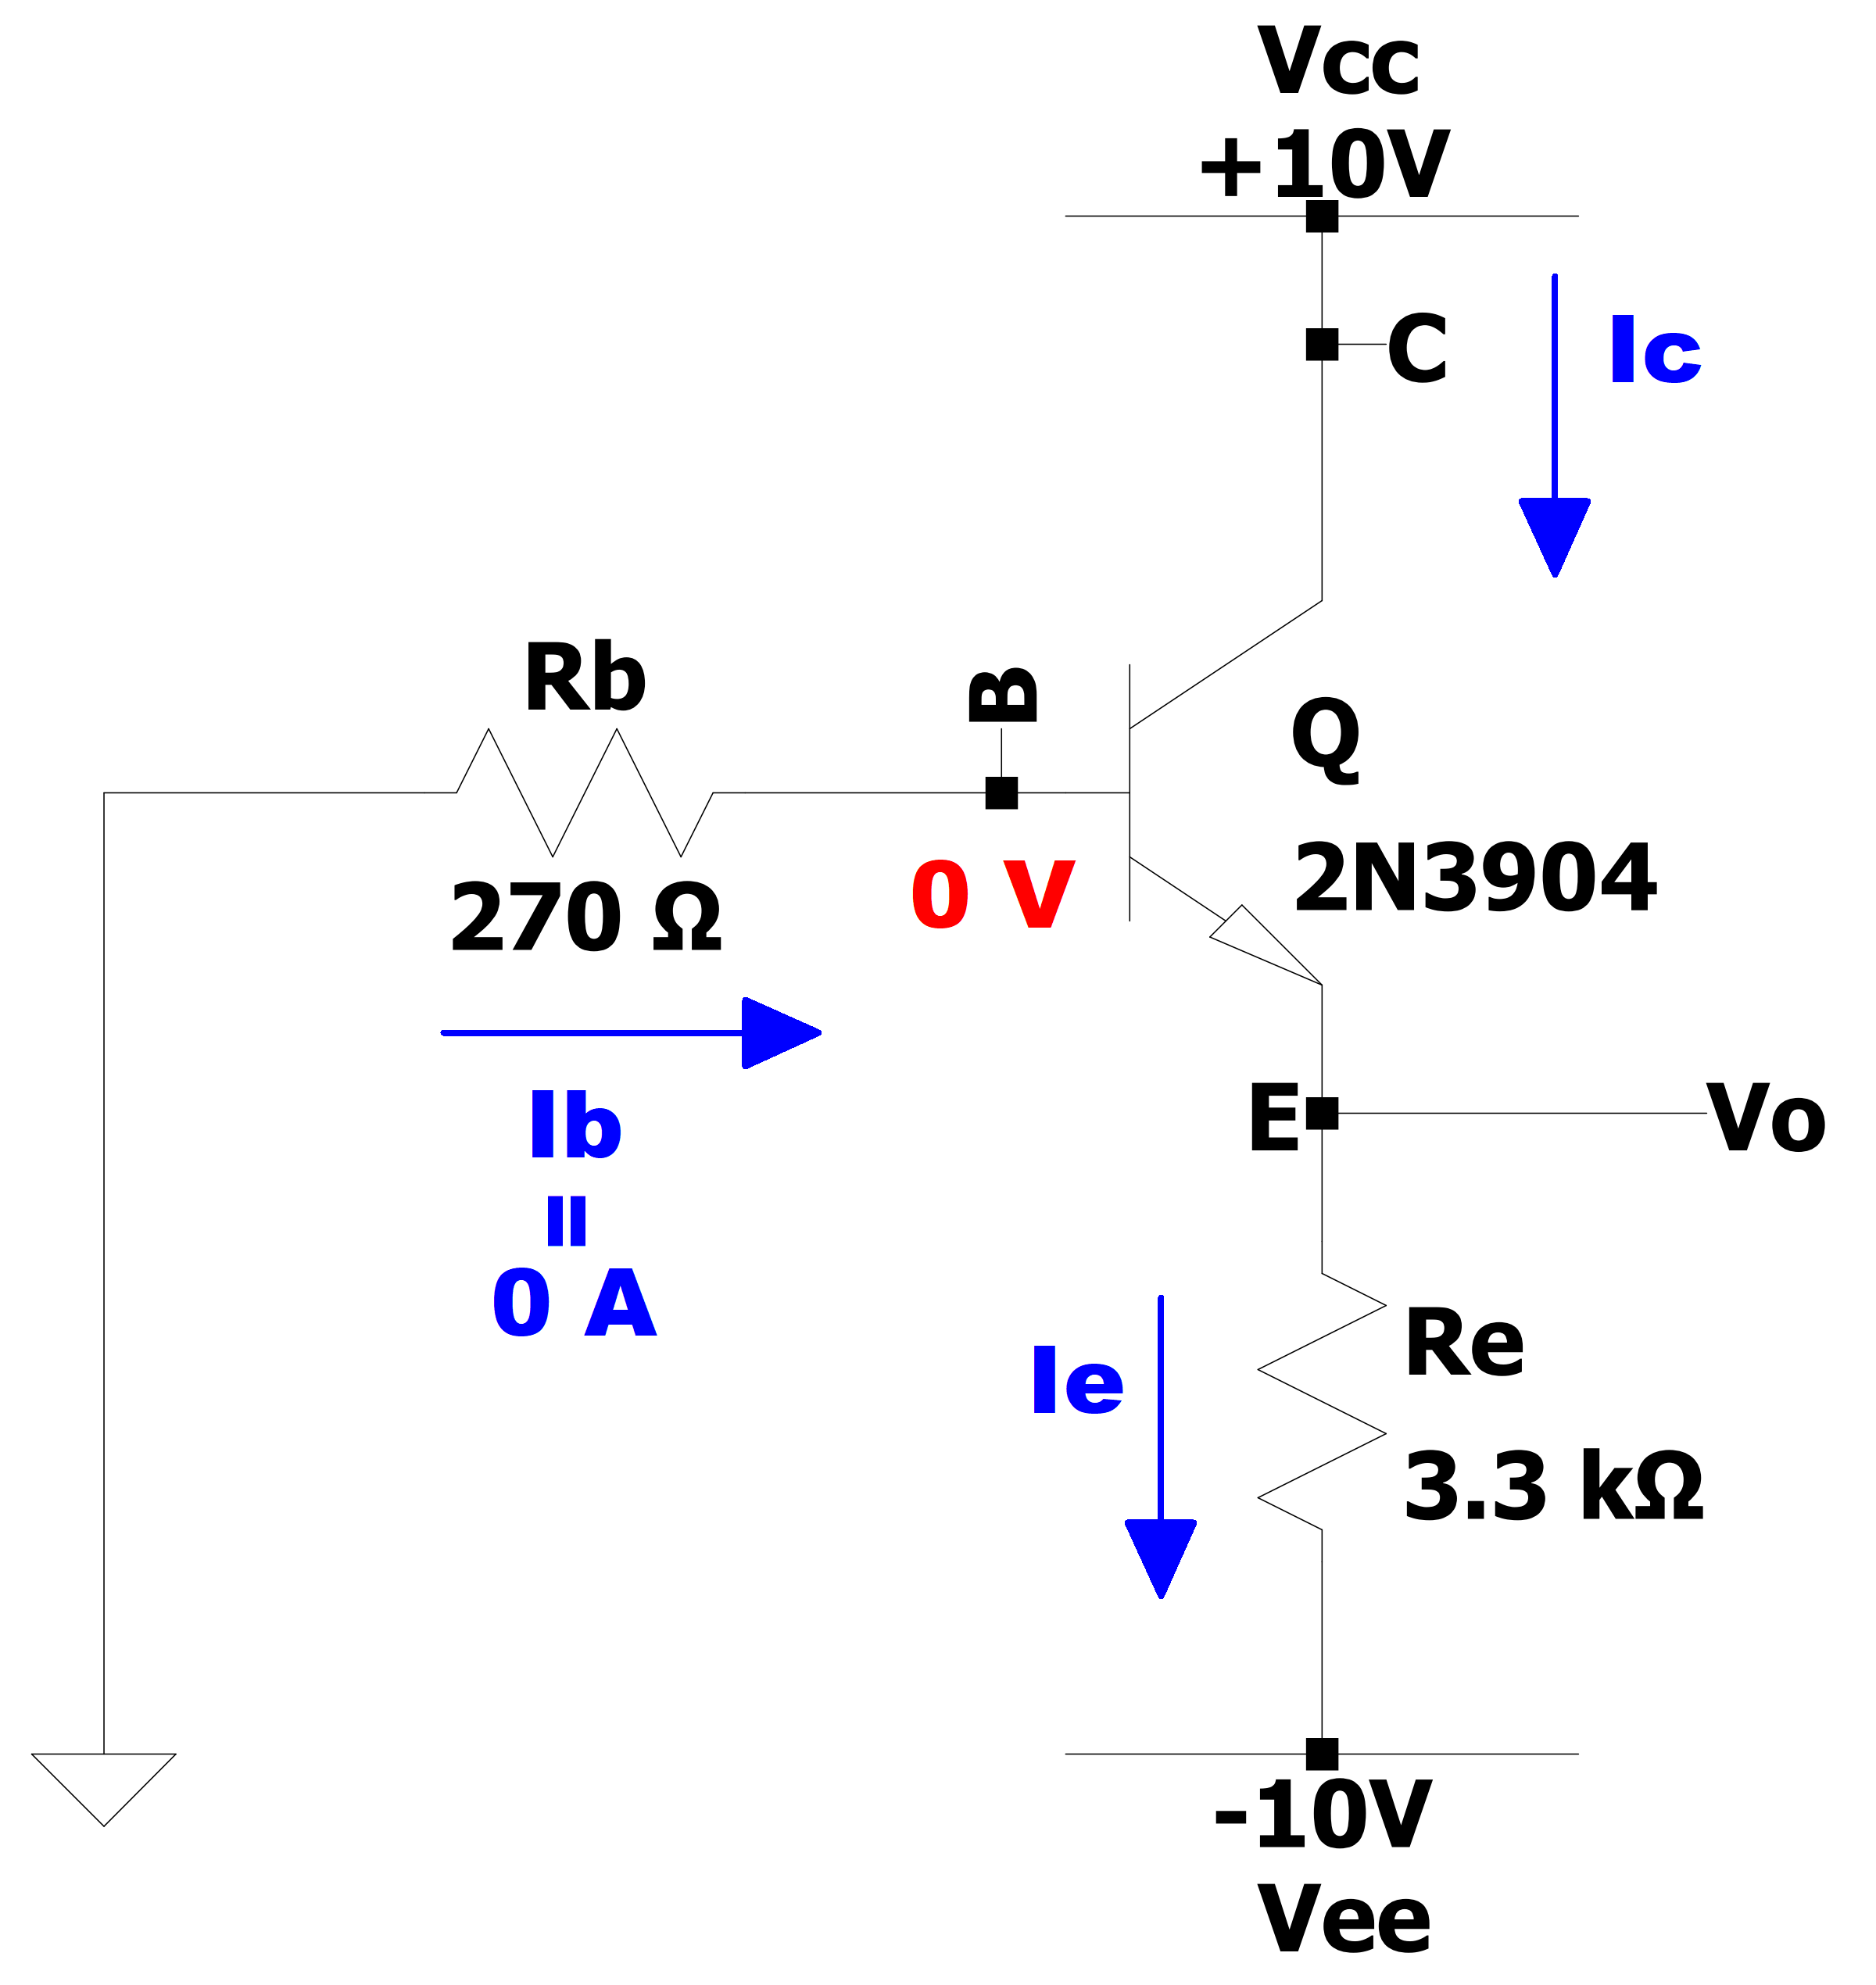
\includegraphics[height=10cm]{immagini/EFv1_pl}
\caption{Punto di lavoro dell'\textit{Emitter follower} ad alimentazione duale.}
\label{figura:EFv1_pl}
\end{figure}
\\Come si vede nell'immagine~\ref{figura:EFv1_pl}, il generatore di segnale $v_{i}$ viene sostituito con un cortocircuito, quindi la resistenza $R_{B}$ si trova fra massa e la base del transistor \textit{Q}. In questo caso non dobbiamo apportare altre modifiche al circuito originale. 
\\Nell'analisi utilizziamo il modello ideale del transistor, perciò assumiamo che $\displaystyle{\beta\rightarrow\infty}$ e che $I_{B}=0A$, di conseguenza la corrente che fluisce nella resistenza è nulla, perciò, per la legge di Ohm, sarà nulla anche la caduta di tensione ai suoi capi, quindi si ricava che $V_{B}=0V$. 
\\Dal bilancio di correnti del  transistor (lo trattiamo come se fosse un nodo) otteniamo che $I_C+I_B=I_E$, ma dato che $I_{B}$ è nulla, allora $I_C=I_E$.
\\Suppondendo che il transistor si trovi in regione attiva diretta, la tensione $V_{BE}$ fra la base e l'emettitore è pari a circa +0.7V perché la giunzione è polarizzata direttamente. Dato che sappiamo che $V_{B}=0V$, possiamo calcolare per differenza $V_{E}$, dunque $V_{E}=-0.7V$. Anche $V_o$ sarà pari a questo valore dato che l'uscita viene prelevata all'emettitore.
\\$V_C$ è pari alla tensione di alimentazione positiva, perciò $V_C=V_{CC}=10V$.
Dato che $V_{CB}>0V$, la giunzione base-collettore è polarizzata inversamente, quindi l'ipotesi che il transistor si trovi in regione attiva diretta è verificata. 
\\Ora possiamo calcolare la corrente di emettitore con la legge di Ohm: 
\\[2pt]\indent$\displaystyle{V_E-V_{EE}=R_E\cdot I_E \rightarrow I_E=I_C=\frac{V_E-V_{EE}}{R_E}=\frac{-0.7V-(-10V)}{3.3k\Omega}=2.818mA}$
\\[2pt]Il circuito è ora completamente risolto, come ultima cosa si può calcolare la transconduttanza che ci servirà successivamente per l'analisi di piccolo segnale. La transconduttanza è definita come rapporto tra la corrente di collettore stazionaria $I_C$ e la tensione termica $V_T$, che a temperatura ambiente vale circa 26mV. 
\\[2pt]In formule: $\displaystyle{g_m=\frac{I_C}{V_T}=\frac{2.818mA}{26mV}=0.108 \frac{A}{V}}$.
\\[3pt]In tabella \ref{table:EFv1_pl} sono riassunte tutte le grandezze ricavate dal punto di lavoro. 
\begin{table}[h]
	\centering
	\begin{tabular}{|c|c|c|c|c|c|c|}
		\hline
		\textbf{V\ped{B}[V]} & \textbf{V\ped{C}[V]} & \textbf{V\ped{E}[V]} & \textbf{I\ped{B}[A]} & \textbf{I\ped{E}[mA]} & \textbf{I\ped{C}[mA]} & \textbf{g\ped{m}[A/V]} \\ 
		\hline
		0 & 10 & -0.7 & 0 & 2.818 & 2.818 & 0.108\\ 
		\hline
	\end{tabular}
\caption{Riassunto delle grandezze ricavate dal punto di lavoro del circuito.}
\label{table:EFv1_pl}
\end{table}
\subsection{Analisi di piccolo segnale} 
Nell'analisi di piccolo segnale bisogna spegnere i generatori di grandezze continue e sostituirli con un cortocircuito se sono generatori di tensione, oppure con un circuito aperto se sono generatori di corrente. Per analisi approssimate, i condensatori sono sostituiti con un cortocircuito e gli induttori con un circuito aperto; per analisi più accurate, invece, non vengono sostituiti e si utilizza la loro impedenza per risolvere il circuito. Infine, i transistor vengono sostituiti con il loro modello per piccolo segnale. Successivamente si va a determinare la tensione di ogni nodo e la corrente che scorre in ogni ramo, esattamente come avveniva per l'analisi del punto di lavoro. 
\begin{figure}[h]
\centering
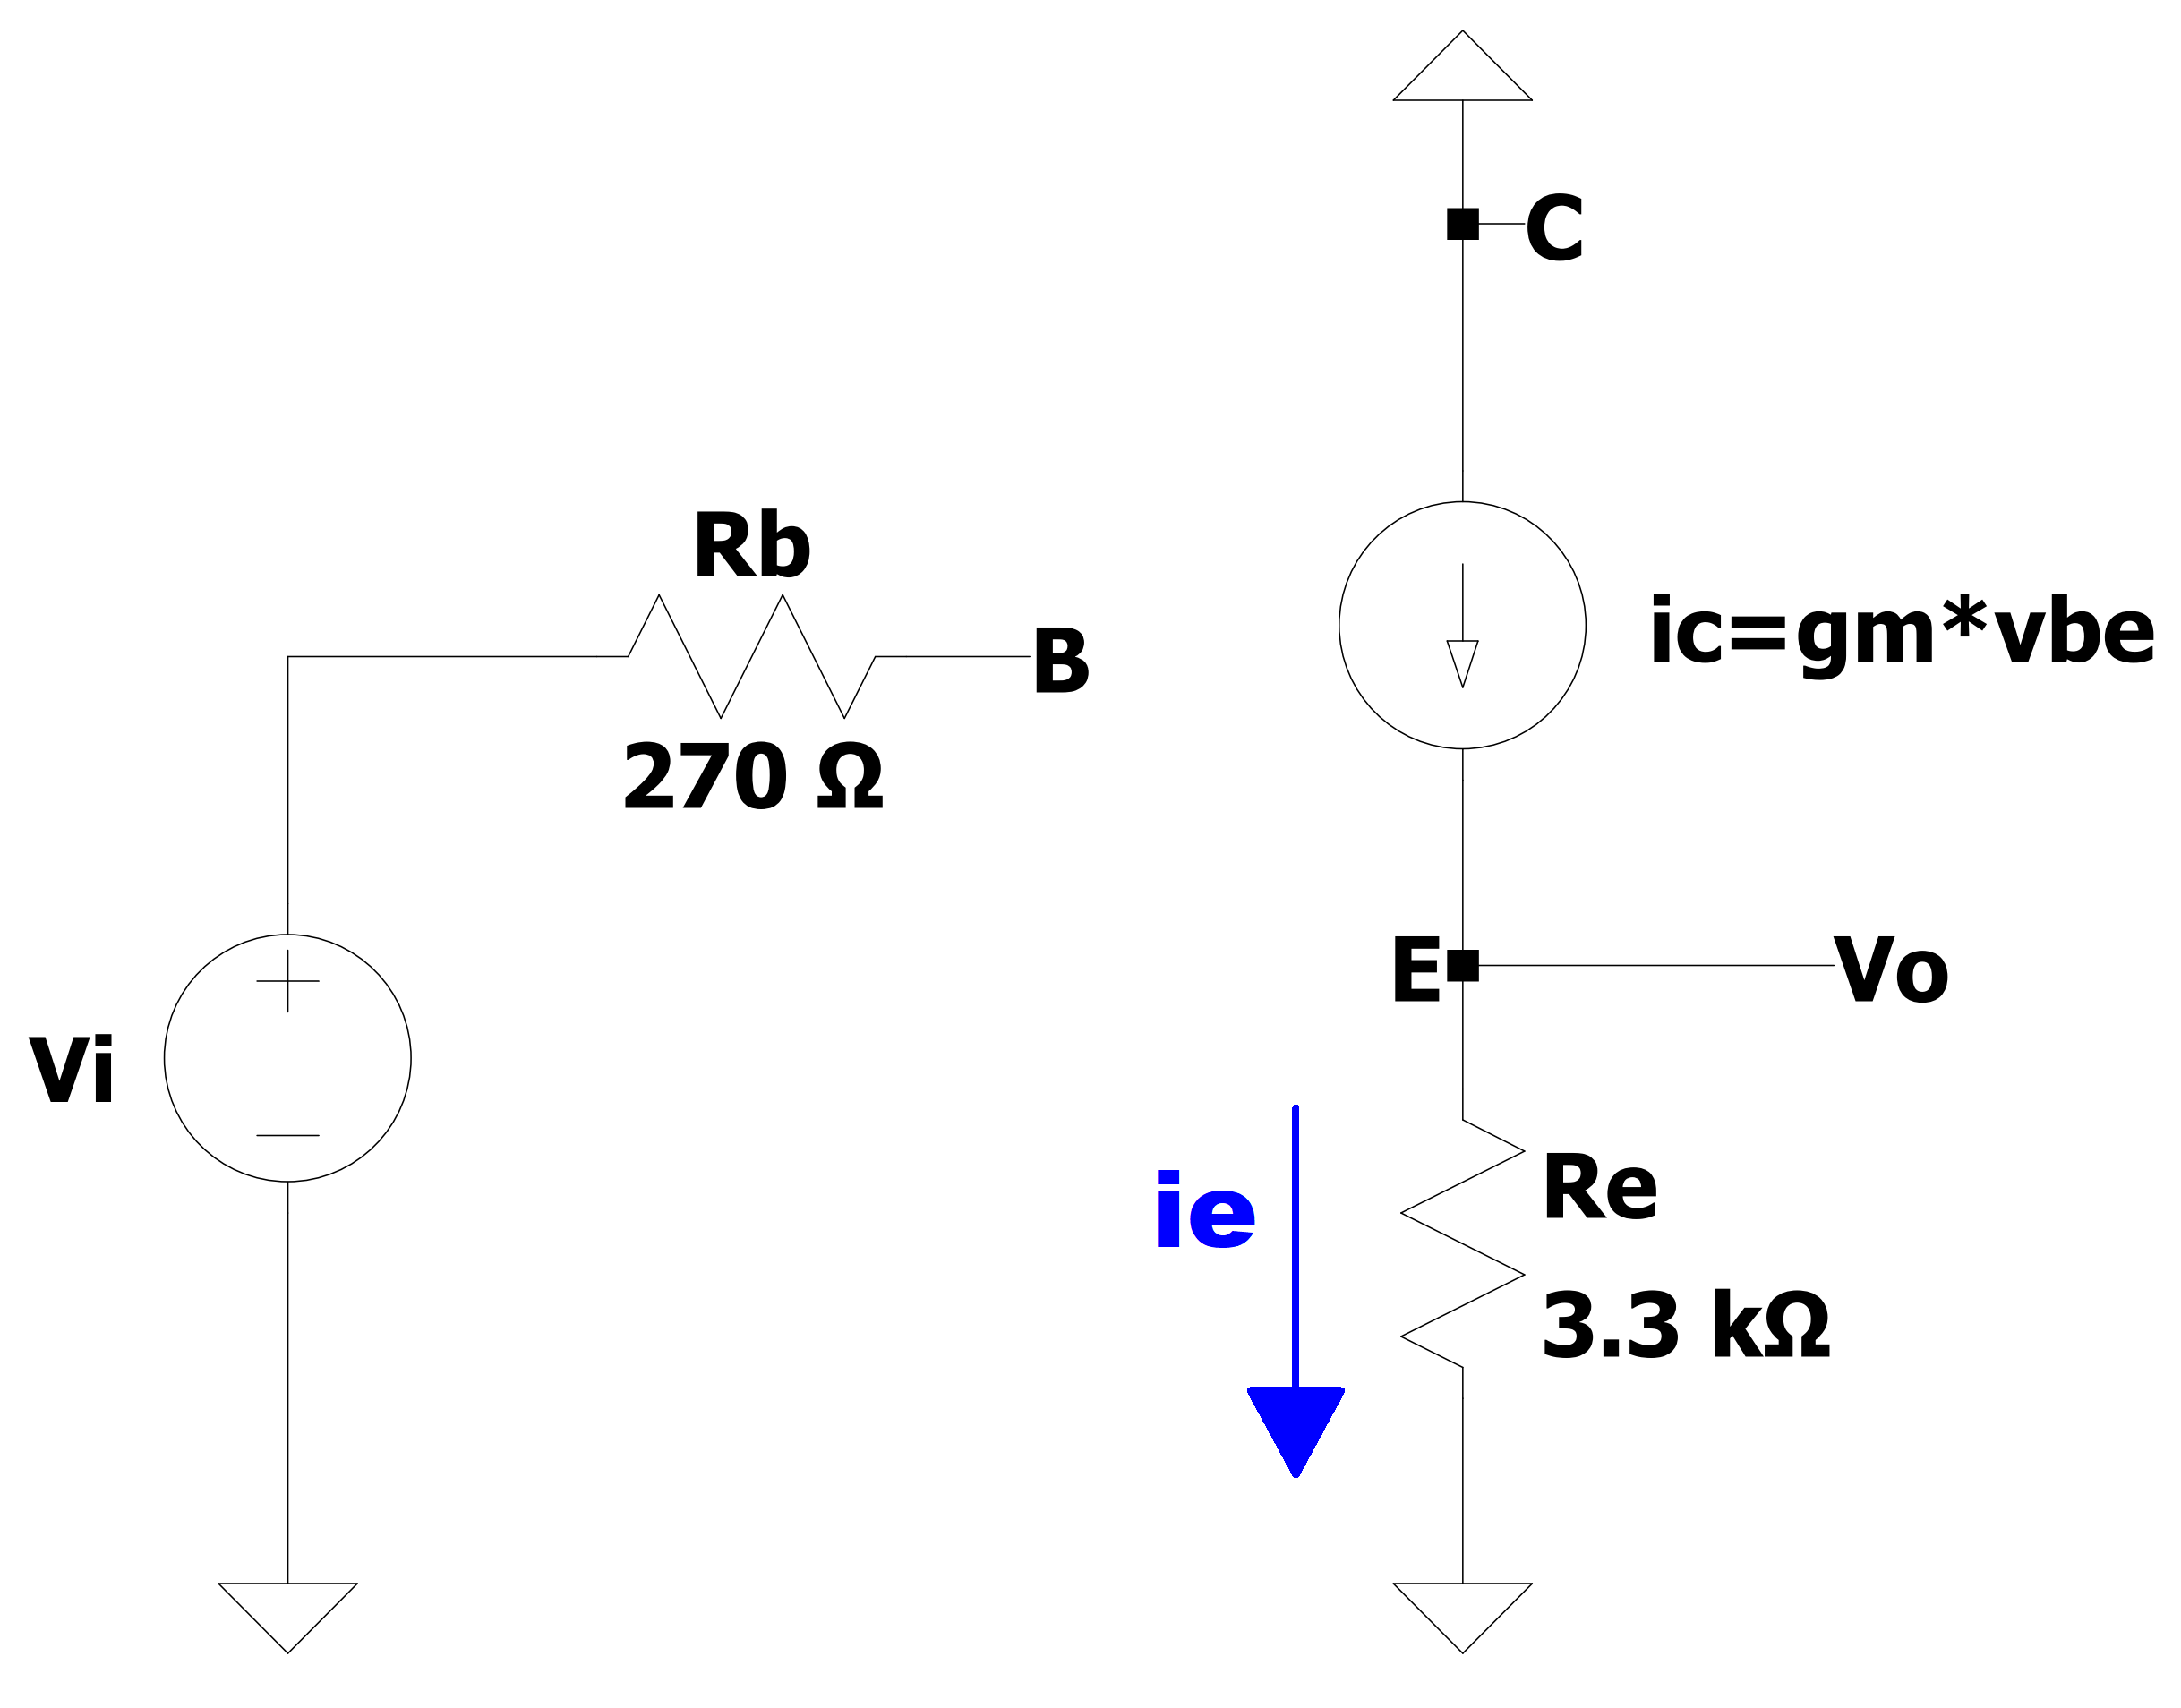
\includegraphics[height=9.6cm]{immagini/EFv1_ps}
\caption{Analisi di piccolo segnale dell'\textit{Emitter follower} ad alimentazione duale.}
\label{figura:EFv1_ps}
\end{figure}
\\Come si può notare dalla figura~\ref{figura:EFv1_ps}, il BJT viene sostituito con il modello per piccolo segnale a bassa frequenza, quindi il terminale di base risulta isolato dal collettore e dall'emettitore, invece questi due terminali sono collegati attraverso un generatore di corrente di valore pari al prodotto fra la transconduttanza $g_m$ e la tensione $v_{BE}$.
\\Dato che la base del transistor è isolata, nel circuito di sinistra non circola corrente, perciò non c'è caduta di tensione sulla resistenza $R_B$, quindi la tensione $v_B$ risulta pari alla tensione applicata in ingresso con il generatore $v_i$.
\\Abbiamo già detto che $i_C=g_m\cdot v_{BE} = g_m(v_B-v_E) $. Ma dato che $v_B=v_i$ e $v_E=v_o$, la formula precedente per il calcolo della corrente di collettore si può riscrivere come $i_C=g_m(v_i-v_o)$.
\\[2pt]Ricaviamo $i_E$ con la legge di Ohm: 
$\displaystyle{i_E=\frac{v_E-0V}{R_E}=\frac{v_o}{R_E}}$.
\\[2 pt] Dal bilancio delle correnti al nodo E otteniamo che $i_C=i_E$. Sostituendo alle due correnti l'espressione ricavata ai punti precedenti ricaviamo la seguente eqauazione:
\\[2pt]\indent $\displaystyle{g_m(v_i-v_o)=\frac{v_o}{R_E}}$.
\\[2pt] A questo punto possiamo ricavare la funzione di trasferimento del circuito manipolando l'espressione ottenuta in precedenza. Questa risulta:
\\[2pt]\indent $\displaystyle{\frac{v_o}{v_i}=\frac{g_mR_E}{1+g_mR_E}\simeq1}$ per $g_mR_E\gg 1$. 
\\[2pt]Allora, si può dire che $v_o=v_i$, ovvero il circuito si comporta come un buffer, come si era già accennato nell'introduzione del circuito.
\subsection{Componenti, strumenti e misure} 
Il circuito, mostrato in figura \ref{figura:fotoEFv1}, è stato realizzato su una breadboard utilizzando questi componenti:
\begin{itemize}
\item transistor bipolare NPN 2N3904;
\item una resistenza da \SI{270}{\ohm} per $R_B$;
\item due resistenze, una da \SI{1.5}{k\ohm} ($R_{E_1}$) ed una da \SI{1.8}{k\ohm} ($R_{E_2}$) connesse in serie, per realizzare la resistenza $R_E$ da \SI{3.3}{k\ohm}.
\end{itemize}
\begin{figure}[h]
\centering
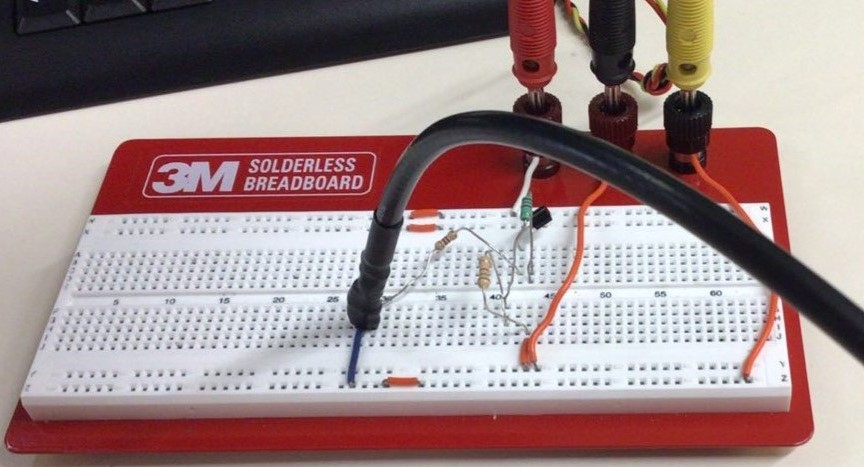
\includegraphics[height=6.6cm]{immagini/fotoEFv1}
\caption{Fotografia del circuito \textit{Emitter follower} ad alimentazione duale realizzato in laboratorio.}
\label{figura:fotoEFv1}
\end{figure}
Per le misure e le analisi, sono stati utilizzati i seguenti strumenti:
\begin{itemize}
\item alimentatore da banco, con alimentazione positiva impostata a 10V ed alimentazione negativa a -10V, entrambe con limite in corrente di 50mA;
\item generatore di forme d'onda;
\item multimetro da banco;
\item oscilloscopio a due canali.
\end{itemize}
Per prima cosa, con il multimetro si sono misurati i valori delle resistenze ed i valori delle tensioni delle giunzioni p-n del transistor (tensione \textit{base-emettitore} e tensione \textit{base-collettore}). I valori ottenuti sono mostrati in tabella \ref{table:EFv1_comp}.
\begin{table}[h]
	\centering
	\begin{tabular}{|c|c|c|}
	\cline{2-3} 
	\multicolumn{1}{c|}{} & \textbf{Valore nominale} & \textbf{Valore misurato}\\ 
		%\hline
		%{} & \textbf{Valore nominale} & \textbf{Valore misurato} \\ 
		\hline
		$\mathbf{R_B}$ & \SI{270}{\ohm} & \SI{271}{\ohm} \\ 
		\hline
		$\mathbf{R_{E_1}}$& \SI{1.5}{k\ohm} & \SI{1.448}{k\ohm} \\ 
		\hline
		$\mathbf{R_{E_2}}$& \SI{1.8}{k\ohm} & \SI{1.788}{k\ohm} \\ 
		\hline
		$\mathbf{V_{BE}}$& $\mathrm{ \simeq0.7V}$ & 0.699V \\ 
		\hline
		$\mathbf{V_{BC}}$& $\mathrm{ \simeq0.7V}$  & 0.659V \\ 
		\hline
	\end{tabular}
	
\caption{Grandezze misurate prima di realizzare il circuito.}
\label{table:EFv1_comp}
\end{table}
\\Le due giunzioni p-n hanno valori di tensione diversi, questo è dovuto alla tecnologia di realizzazione del BJT: essendo un dispositivo planare, le due giunzioni hanno lunghezza diversa, di conseguenza anche il loro valore di tensione sarà diverso. Il valore totale della resistenza $R_E$ è pari a \SI{3.236}{k\ohm}, poco meno del 2\% rispetto al suo valore nominale che è \SI{3.3}{k\ohm}.
\\\indent Dopo aver posizionato tutti i componenti sulla breadboard, è stato fatto lo studio del punto di lavoro del circuito. Non è stato applicato il segnale e il terminale della resistenza $R_B$ non connesso alla base del transistor è stato collegato a massa. Il circuito risultante è mostrato in figura \ref{figura:fotoEFv1_pl}.
\begin{figure}[h]
\centering
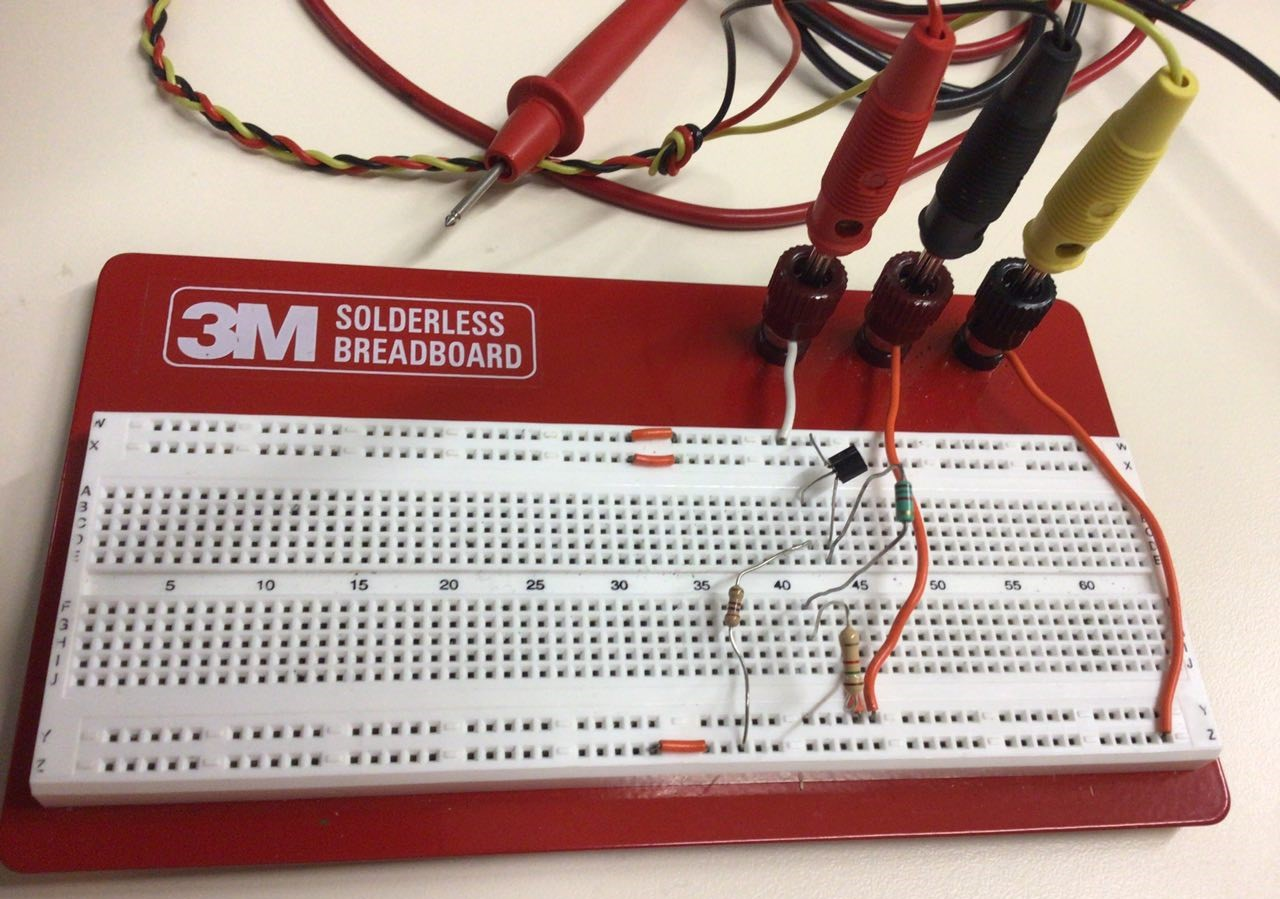
\includegraphics[height=7.3cm]{immagini/fotoEFv1_pl}
\caption{Fotografia del circuito \textit{Emitter follower} con le connessioni per lo studio del punto di lavoro.}
\label{figura:fotoEFv1_pl}
\end{figure}
\\Le tensioni sono state misurate con il multimetro da banco, le correnti di base e di emettitore sono state ricavate utilizzando la legge di Ohm, mentre la corrente di collettore è stata calcolata per differenza dalle altre due correnti. I risultati sono mostrati in tabella \ref{table:EFv1_pl_mis}. 
\begin{table}[h]
	\centering
	\begin{tabular}{|c|c|c|c|c|c|c|}
		\hline
		\textbf{V\ped{B}[mV]} & \textbf{V\ped{C}[V]} & \textbf{V\ped{E}[V]} & \textbf{I\ped{B}[mA]} & \textbf{I\ped{E}[mA]} & \textbf{I\ped{C}[mA]} & \textbf{g\ped{m}[A/V]} \\ 
		\hline
		-3.515 & 10.000 & -0.687 & 0.013 & 2.878 & 2.865 & 0.108\\ 
		\hline
	\end{tabular}
\caption{Grandezze misurate dallo studio del punto di lavoro del circuito.}
\label{table:EFv1_pl_mis}
\end{table}
\\I valori ottenuti sono confrontabili con i risultati teorici calcolati nella sezione \ref{puntolavoroEFv1}. La differenza principale è che sia $V_B$ che $I_B$ non sono nulle, anche se il loro valore (in modulo) è molto piccolo. In particolare, dato che la corrente $I_B$ è piccola, l'approssimazione adottata nello studio teorico del circuito di trascurarla è ragionevole. 
\\\indent Dopo lo studio del punto di lavoro del circuito, è stato applicato in ingresso il segnale collegando con un cavo BNC il generatore di forme d'onda al circuito. Il circuito risultante è quello già mostrato in figura \ref{figura:fotoEFv1}. La forma d'onda utilizzata è una sinusoide con tensione picco-picco $V_{PP}$ di 1V e frequenza $f$ pari a \SI{1}{k\hertz}. 
\\\indent Per visualizzare graficamente la tensione in ingresso e la tensione in uscita è stato utilizzato l'oscilloscopio. Entrambe le sonde sono state collegate a massa con il coccodrillo, la punta di una sonda è stata collegata alla base del transistor (canale 1, traccia gialla) mentre la punta dell'altra sonda è stata collegata all'emettitore (canale 2, traccia azzurra). Il grafico è visibile in figura \ref{figura:oscillo1}.
\begin{figure}[h]
\centering
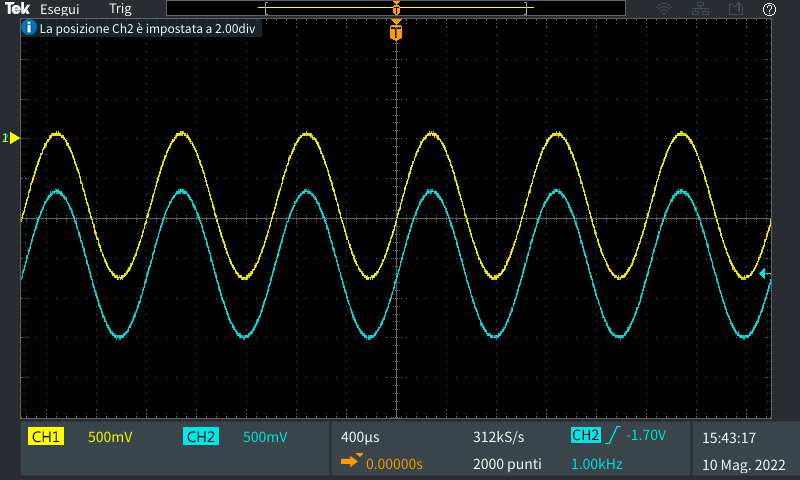
\includegraphics[height=7cm]{immagini/oscillo1}
\caption{Grafico della tensione in ingresso (CH1) e della tensione in uscita (CH2) al circuito.}
\label{figura:oscillo1}
\end{figure}
\\
Com'è possibile vedere dal grafico, il guadagno del circuito è unitario perché entrambe le sinusoidi hanno la stessa ampiezza. La tensione applicata in ingresso la misuriamo in uscita con una differenza di circa 0.7V, che è la caduta di tensione data dalla giunzione p-n fra base ed emettitore. I due segnali sono in fase. 
\\\indent In realtà, il guadagno del circuito non è esattamente unitario e nemmeno lo sfasamento, o offset, è proprio nullo, come invece sembrerebbe dal grafico precedente. La tensione in uscita è legata alla tensione in ingresso da una relazione del tipo $y=a+bx$, dove $y$ è la tensione in uscita, $x$ la tensione in ingresso, $a$ l'offset e $b$ il guadagno del circuito. Per ricavare il valore dei parametri $a$ e $b$ sono state applicate in ingresso al circuito diverse sinusoidi, tutte di frequenza \SI {1}{k\hertz} ma di ampiezza variabile. La tensione picco-picco è infatti stata variare da 0.5V a 5.0V con step di 0.5V. Successivamente, con l'oscilloscopio, si sono misurati i valori di tensione picco-picco in ingresso, $V_{PP_i}$, e in uscita, $V_{PP_o}$. 
\\\indent Per ridurre l'effetto dei disturbi e del rumore sulle misure, i segnali sono stati filtrati con un passa-basso con frequenza di taglio di \SI{20}{M\hertz}, poi sono stati mediati utilizzando 16 acquisizioni. Facendo così, il valore misurato dall'oscilloscopio risulta molto più stabile. Le misure sono riportate in tabella \ref{table:tabgrafico}.
\begin{table}[h]
	\centering
	\begin{tabular}{|c|c|}
		\hline
		$\mathbf{V_{PP_i}[V]}$ & $\mathbf{V_{PP_o}[V]}$\\ 
		\hline
		0.503 & 0.505 \\
		\hline
		1.000 & 1.006 \\
		\hline
		1.497 & 1.506 \\
		\hline
		1.989 & 2.002 \\
		\hline
		2.486 & 2.502 \\
		\hline
		2.978 & 3.001 \\
		\hline
		3.473 & 3.496 \\
		\hline
		3.965 & 3.993 \\
		\hline
		4.461 & 4.497 \\
		\hline
		4.951 & 4.985 \\
		\hline
	\end{tabular}
\caption{Valori della tensione picco-picco in ingresso e in uscita al circuito.}
\label{table:tabgrafico}
\end{table}
\\I dati della tabella precedente sono stati elaborati su MATLAB per ricavare la retta di regressione che ci permette di stimare i valori di $a$ e $b$. Nel grafico seguente, la figura \ref{figura:graficoEFv1}, si riportano le misure, la retta interpolata e la retta teorica. 
\begin{figure}[h]
\centering
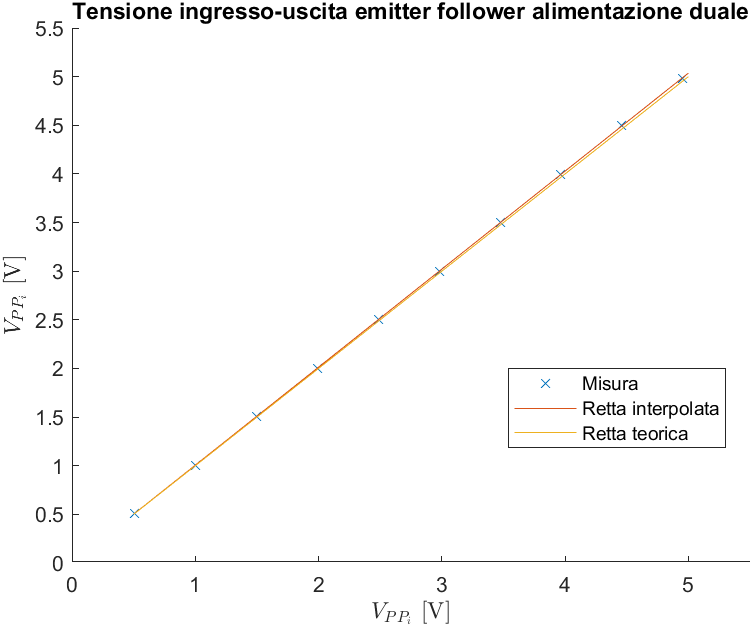
\includegraphics[height=7cm]{immagini/graficoEFv1}
\caption{Confronto grafico fra la tensione ingresso-uscita interpolata e quella teorica.}
\label{figura:graficoEFv1}
\end{figure}
\\L'equazione della retta interpolata è: $y=-0.0020949+1.0077x$. Il risultato è chiaramente in disaccordo con la teoria, perché sebbene il guadagno è molto prossimo all'unità, non può essere maggiore, perché questo significherebbe che il circuito eroga più energia rispetto a quella fornita in ingresso. Il motivo di questo risultato anomalo può essere dovuto alla regolazione non sufficientemente precisa della capacità di compensazione della sonda collegata al secondo canale dell'oscilloscopio.
\section{Seconda versione} % alimentazione singola
\subsection{Punto di lavoro} 
\subsection{Analisi di piccolo segnale}  % versione base + versione partitore + versione condensatore
\subsection{Componenti, strumenti e misure} 


%----------------------------------------------------------------------------------------
%	CIRCUITO 2: COMMON EMITTER AMPLIFIER
%----------------------------------------------------------------------------------------
\clearpage
\newpage
\chapter{Circuito 2: Common Emitter Amplifier}
\section{Introduzione} 
\section{Prima versione} % senza degenerazione emitter, solo trattazione teorica non realizzato in lab
\subsection{Schema} %?mettere
\subsection{Analisi del circuito} 
\section{Seconda versione} % con degenerazione emitter, alimentazione duale
\subsection{Punto di lavoro} 
\subsection{Analisi di piccolo segnale} 
\subsection{Componenti, strumenti e misure} 
\section{Terza versione} % con degenerazione emitter, alimentazione singola (in piccolo segnale aggiungi già il condensatore)
\subsection{Punto di lavoro} 
\subsection{Analisi di piccolo segnale}  
\subsection{Componenti, strumenti e misure} 


%----------------------------------------------------------------------------------------
%	CIRCUITI 3 E 4: AMPLIFICATORE OPERAZIONALE \mu A741
%----------------------------------------------------------------------------------------
\clearpage
\newpage
\chapter{Circuiti 3 e 4: Amplificatore operazionale \textmu A741}
\section{Introduzione} 
\section{Amplificatore invertente} 
\subsection{Schema} %?mettere
\subsection{Analisi del circuito} 
\subsection{Componenti, strumenti e misure} 
\section{Integratore} 
\subsection{Schema} %?mettere
\subsection{Analisi del circuito} 
\subsection{Componenti, strumenti e misure} 





%----------------------------------------------------------------------------------------

\end{document}
